\documentclass{article}
\usepackage{tikz}
\usetikzlibrary{matrix, arrows.meta, positioning}

\begin{document}

\begin{figure}[h]
    \centering
    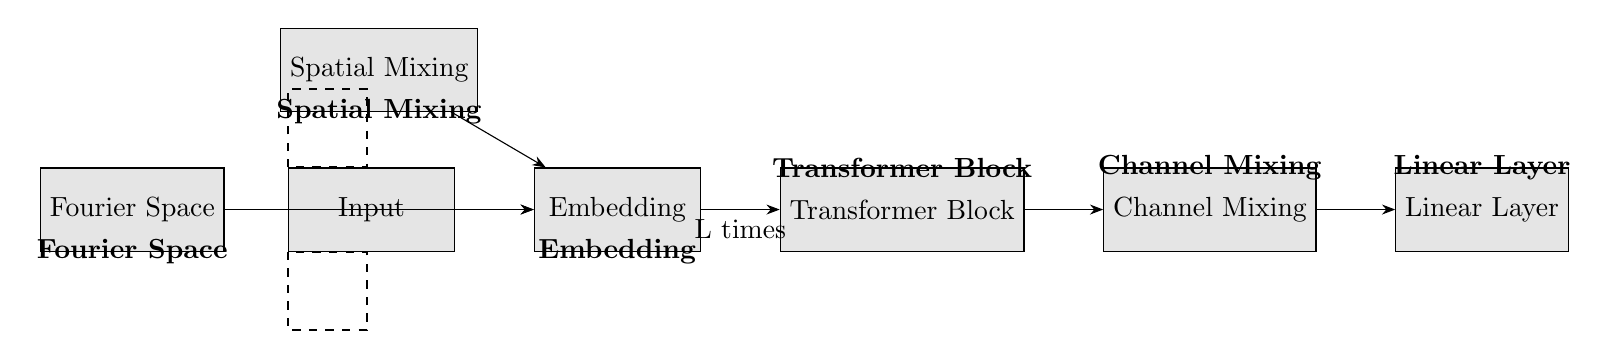
\begin{tikzpicture}[node distance=1cm, auto]
        % Define styles
        \tikzset{
            block/.style = {draw, fill=gray!20, rectangle, minimum height=3em, minimum width=6em},
            line/.style = {draw, -Stealth},
            cloud/.style = {draw, ellipse,fill=red!20, minimum height=2em},
        }
        
        % Input layer
        \node [block] (input) {Input};
        
        % Embedding layer
        \node [block, right=of input] (embedding) {Embedding};
        
        % Transformer Block
        \node [block, right=of embedding] (transformer_block) {Transformer Block};
        \node [block, right=of transformer_block] (channel_mixing) {Channel Mixing};
        \node [block, right=of channel_mixing] (linear_layer) {Linear Layer};
        
        % Arrows
        \draw [line] (input) -- (embedding);
        \draw [line] (embedding) -- node[below] {L times} (transformer_block);
        \draw [line] (transformer_block) -- (channel_mixing);
        \draw [line] (channel_mixing) -- (linear_layer);
        
        % Additional elements
        \node [block, above left=of embedding] (spatial_mixing) {Spatial Mixing};
        \node [block, below left=of spatial_mixing] (fourier_space) {Fourier Space};
        
        \draw [line] (spatial_mixing) -- (embedding);
        \draw [line] (fourier_space) -- (embedding);
        
        % Dashed lines
        \draw [dashed, thick] (input.north west) -- ++(0, 1) -- ++(1, 0) -- ++(0, -1) -- ++(-1, 0) -- cycle;
        \draw [dashed, thick] (input.south west) -- ++(0, -1) -- ++(1, 0) -- ++(0, 1) -- ++(-1, 0) -- cycle;
        
        % Labels
        \node at (embedding.south) {\textbf{Embedding}};
        \node at (transformer_block.north) {\textbf{Transformer Block}};
        \node at (channel_mixing.north) {\textbf{Channel Mixing}};
        \node at (linear_layer.north) {\textbf{Linear Layer}};
        \node at (spatial_mixing.south) {\textbf{Spatial Mixing}};
        \node at (fourier_space.south) {\textbf{Fourier Space}};
    \end{tikzpicture}
    \caption{Overview of the used architecture based on the FourCastNet model \cite{pathak2022fourcastnet}. We initialize the model from pre-trained weights \cite{fcn_weights} and replace the weather-specific head with a linear head for modelling the normalized difference vegetation index (NDVI).}
    \label{fig:architecture}
\end{figure}

\end{document}